\subsection{Thermodynamics in (re-)entry vehicles}\label{sec:thermo}
Thermodynamics is used to ensure that components of the reentry vehicle stay within a certain temperature range. These temperature ranges are a function of the intended use of the components and material selection. This literature review is broken down in three major parts. The first briefly explains the principles needed to describe the transfer of heat within structures. The second concerns the heat shield needed for the reentry phase, which is heavily linked to the aerodynamics. This is split up in non-inflatable and inflatable heat shields. The third deals with the thermal control of the capsule itself. For example, the temperature inside the capsule should be suitable for human payloads.

\subsubsection{Thermodynamic principles}
At the start of the mission the reentry vehicle can be seen as a closed system that has a total energy (\gls{sym:E}) in the form of internal energy (\gls{sym:U}), kinetic energy (\gls{sym:KE}) and potential energy (\gls{sym:PE}). For successful reentry the kinetic and potential must be reduced. This can be done by transferring the energy across the boundary of the system. There are three methods to transfer the energy. Energy transfer by heat, by work and by mass flow. The latter requires the system to be open such that mass is allowed to leave the system \cite{Cengel2010}. An example of energy transfer by heat is the heating of gas near the wall of the heat shield and heating of the heat shield itself. Energy transfer by work could for example be the work done by the skin friction drag. The use of thrusters is an example of energy transfer due to mass flow as the propellant mass flows out of the open system. 

Energy transfer by heat, or simply heat transfer, has three modes: conduction, convection and radiation. Conduction is the transfer of heat between particles of a material due to interactions between these particles. Convection is the transfer of heat between a solid surface and a moving fluid. Radiation is transfer of heat due to the emission of electromagnetic energy from a surface to its surroundings \cite{Cengel2010, Karam1998}. Each of these modes can be described by governing equations as described in Ref.\cite{Holman2002}. Radiation is given by the Stefan-Boltzmann law and conduction by Fourier's law \cite{Cengel2010, Holman2002}.

\subsubsection{Thermal protection system}
The thermodynamic principles can be used to design a heat shield. The design of such a heat shield, also called a \acrfull{tps}, depends on several parameters. In general it all comes down to the trajectory the reentry vehicle will follow. The steeper the reentry trajectory, the larges the deceleration and the more g-loads will be endured by the (human) payload. The reentry vehicle will have a nominal trajectory with deviations. An overshoot results in a longer descent and can result in skipping off the planet, whereas an undershoot will result in a high descent rate. The larger the overshoot angle, the longer the reentry vehicle will be in atmosphere an thus creating a higher heat loading on the structure. On the other hand, for a larger undershoot angle, the heat development over time will be faster inducing a larger heat flux on the system. Also, the undershoot angle determines the trajectory with the highest dynamic pressure, which is important for structural sizing. 

Not only the trajectory is important for the design, but also the shape with its bluntness. The bigger the heat shield and the larger the bluntness, the more the  thermal loads can be distributed over the capsule. This will result in a thinner \gls{tps} such that less mass is needed. This can cause aerodynamic instability, however \cite{Smoot}.

The temperature development in the structure through multiple layers of material can be determined when the heat loading and heat flux is known. An example of a method to determine the heat development is given by \cite{Daryabeigi2002}.

\paragraph{Heat shield for non-inflatable structures}
Throughout the last century several reentry attempts have been performed with different \gls{tps}s. This paragraph and the next paragraph focus on several concepts. This paragraph focuses on non-inflatable solutions and the next on inflatables. 

A typical \gls{tps} example of a non-inflatable structure is the \gls{tps} of the reentry vehicle of the Apollo mission \cite{Pavlosky1974}. Different from inflatables, the \gls{tps} of the Apollo also has an aft shield and a crew compartment heat shield, because the front shield cannot deflect the direct flow from the sides and the aft part of the structure. An overview of the \gls{tps} lay-up is shown in figure \ref{fig:tpslayupapollo}. It consist of an ablative layer, which is sacrificed during reentry. The second layer is brazed stainless steel. This layer is followed by an insulator to keep the temperature difference between the outer layers and the inner layers. Last but not least, the connection to the rest of the structure is an aluminum honeycomb structure.

\begin{figure}[H]
\centering
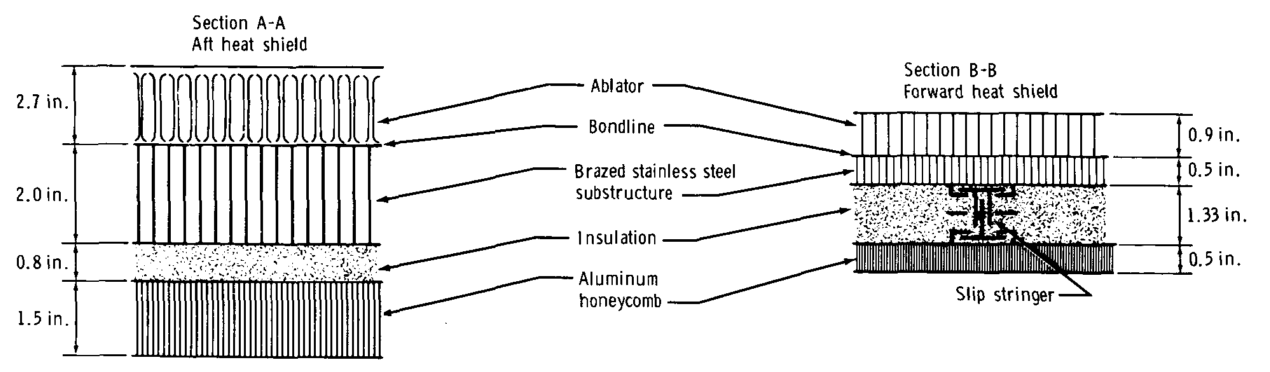
\includegraphics[width = 0.55\textwidth]{Figure/tpsApollo.png}
\caption[Example of the \gls{tps} lay-up for the Apollo reentry vehicle]{Example of the \gls{tps} lay-up for the Apollo reentry vehicle \cite[p.5]{Pavlosky1974}.}
\label{fig:tpslayupapollo}
\end{figure}

\paragraph{Heat shield for inflatable structures}
The usage of  an inflatable structure is preferable over a non-inflatable structure for several reasons. An inflatable heat shell is not directly limited to the size of the launcher. Therefore a much larger diameter of the \gls{tps} can be obtained. This is an advantage because the heat loads on the structure can be distributed resulting in a lower front shell mass. Furthermore, the heat at the back side of the vehicle will be severely lower, such that there is no need for a back shell \cite{Hughes2005}. Therefore, less mass is needed and less effort needs to be done to verify and validate the thermal loads on payload closely located to the back shell. Although the system is very promising in terms of mass, the system does add a lot of complexity. 

The \gls{tps} of the IRVE vehicles consists of several layers \cite{Litton2011} which are shown in Figure \ref{fig:tpslayup} similar to the before mentioned Figure \ref{fig:matlayup}. The outer layer protects the structure from the direct incoming flow by distributing and absorbing or dissipating the heat. Also, it will carry the shearing loads from the flow. The second layer is an insulator and keeps the temperature behind the shield at a low level. Finally, the last Kevlar layer provides a fabric connection between the heat shield and the rest of the structure and carries most of the structural loads. The Kapton in this layer is an impermeable layer and keeps hot gases from passing this layer.

\begin{figure}[H]
\centering
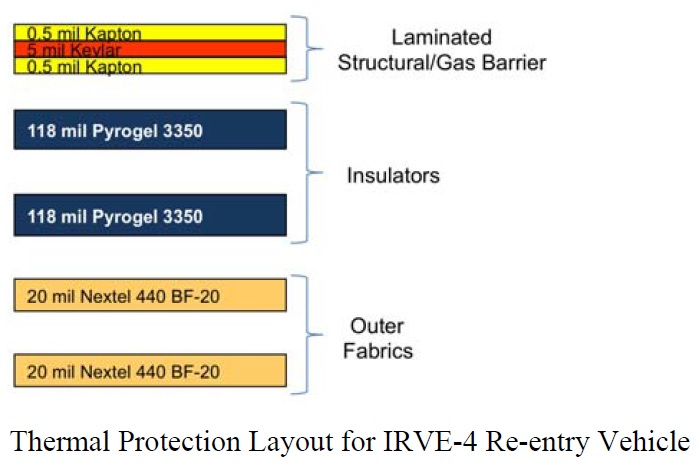
\includegraphics[width = 0.55\textwidth]{Figure/IRVE4TPS.jpg}
\caption[Example of the \gls{tps} lay-up for the IRVE-4 reentry vehicle]{Example of the \gls{tps} lay-up for the IRVE-4 reentry vehicle\cite[p.6]{Litton2011}.}
\label{fig:tpslayup}
\end{figure}

There has not yet been an actual entry on Mars with an inflatable shield, but \gls{nasa} has demonstrated a well verified and validated concept \cite{Dillman2010, Dillman2012}. Another non-verified concept is the use of ballutes, which can be applied in case of high mass transportation \cite{Hall2001}. Due to its large size the thermal loads on the structure are small. However, the capsule, located in front of the ballute is exposed to a the free flow and needs additional thermal protection.

\subsubsection{Thermal control system}
For the \gls{tcs} of the crew capsule the book on Thermal Control by R. Karam is leading\cite{Karam1998}. Karam explains that heat fluxes due to conduction and radiation can be related to temperature using certain proportionality factors that depend on physical constants, material properties, surface conditions, geometry and temperature. The purpose of thermal control is to change the proportionality factors such that the desired temperature range is reached and retained. The changing of the proportionality factors is done by proper selection of materials and configurations.

The actual \gls{tcs} is divided into two parts, namely passive and active thermal control. The distinction is made whether the control component uses power or not. For example the use of insulation is a form of passive thermal control. Radiators and heaters are examples of active thermal control. Also a hot and cold case are considered to define the upper and lower limits for the temperatures. The hot case has the maximum possible influx of heat during the mission and the cold case the minimum possible influx of heat during the mission. Naturally these limits should lie within the desired temperature range. If this is not the case, the \gls{tcs} should be improved \cite{Karam1998}.

Karam also describes how to perform thermal analysis using thermal models, which can be used in combination with Holman's book on heat transfer \cite{Holman2002}. The predictions made in the thermal analysis rely on the law of conservation of energy. Both books (\cite{Karam1998,Holman2002}) describe how to do the analysis with computational methods, where Holman elaborates more on the use of a grid to find the thermal distributions at certain times. In this way the \gls{tcs} can be verified by analysis.




